%\VignetteIndexEntry{brainstars}
%\VignetteDepends{brainstars}
%\VignetteKeywords{brainstars}
%\VignettePackage{brainstars}
\documentclass[12pt,fullpage]{article}

\usepackage{amsmath,epsfig,pstricks,fullpage}
\usepackage{hyperref}
\usepackage{url}
\usepackage[authoryear,round]{natbib}

\newcommand{\Rfunction}[1]{{\texttt{#1}}}
\newcommand{\Robject}[1]{{\texttt{#1}}}
\newcommand{\Rpackage}[1]{{\textit{#1}}}
\newcommand{\Rclass}[1]{{\textit{#1}}}
\newcommand{\Rmethod}[1]{{\textit{#1}}}

\author{Itoshi Nikaido$^\ddagger$\footnote{dritoshi@gmail.com} \and Takeya Kasukawa$^\ddagger$\footnote{kasukawa@gmail.com}}
\usepackage{Sweave}
\begin{document}
\title{Using the BrainStars package}
\maketitle
\begin{center}$^\ddagger$The RIKEN Center for Developmental Biology
\end{center}

\tableofcontents

%%%%%%%%%%%%%%%%%%%%%%%%%%%%%%%%%%%%%%%%%%%%%%
\section{Overview of BrainStars} 

BrainStars is a quantitative expression database of the adult
mouse brain. The database has genome-wide expression profile at 51
adult mouse CNS regions.

For 51 CNS regions, slices (0.5-mm thick) of mouse brain were cut on a
Mouse Brain Matrix, frozen, and the specific regions were punched out
bilaterally with a microdissecting needle (gauge 0.5 mm) under a
stereomicroscope. For each region, we took samples every 4 hours,
starting at ZT0 (Zeitgaber time 0; the time of lights on), for 24
hours (6 time-point samples for each region), and we pooled the
samples from the different time points. We independently sampled each
region twice (n=2).

These samples were purified their RNA, and measured with Affymetrix
GeneChip Mouse Genome 430 2.0 arrays. Expression values were then
summarized with the RMA method. After several analysis with the
expression data, the data and analysis results were stored in the
BrainStars database.

BrainStars database has a REST API to query gene expression data, 
annotations and some kind of figures written by Dr. Takeya Kasukawa. 
This package is wrapper for BrainStars REST API in R. BrainStars data, 
images and texts (excluding ABA data and images) are licensed under a 
Creative Commons Attribution 2.1 Japan License.
  
\section{Getting Started using BrainStars package}
\subsection{Getting expression profiles by ProbeSet IDs}
Getting expression data from BrainStars is easy.  \Rfunction{getBrainStarsExpression} 
aquires gene expression profile and then parse the data into \Rclass{ExpressionSet} 
object.  Usage is quite simple:

\begin{Schunk}
\begin{Sinput}
> library(brainstars)
\end{Sinput}
\end{Schunk}

This loads the brainstars library.

\begin{Schunk}
\begin{Sinput}
> my.eset <- getBrainStarsExpression("1439627_at")
\end{Sinput}
\end{Schunk}

Now, \Robject{my.eset} contains the R data structure (of class \Rclass{ExpressionSet}) that represents the entry 1439627\_at from BrainStars.

The function \Rfunction{getBrainStarsExpression} accepts vector of mutiple probeset IDs.
\begin{Schunk}
\begin{Sinput}
> ids <- c("1439627_at", "1439631_at", "1439633_at")
> my.esets <- getBrainStarsExpression(ids)
> my.esets
\end{Sinput}
\begin{Soutput}
ExpressionSet (storageMode: lockedEnvironment)
assayData: 3 features, 102 samples 
  element names: exprs 
protocolData: none
phenoData: none
featureData: none
experimentData: use 'experimentData(object)'
Annotation:  
\end{Soutput}
\end{Schunk}

You can access the matrix of expression in the following method:
\begin{Schunk}
\begin{Sinput}
> my.mat <- exprs(my.esets)
\end{Sinput}
\end{Schunk}

\subsection{Getting figures}
We can retrieve some kind of barplots and brain map images from BrainStars.

\begin{Schunk}
\begin{Sinput}
> getBrainStarsFigure("1439627_at", "exprgraph", "png")
\end{Sinput}
\begin{Soutput}
Save figure file at 1439627_at.exprgraph.png 
\end{Soutput}
\begin{Sinput}
> getBrainStarsFigure("1439627_at", "exprmap", "pdf")
\end{Sinput}
\begin{Soutput}
Save figure file at 1439627_at.exprmap.pdf 
\end{Soutput}
\begin{Sinput}
> getBrainStarsFigure("1439627_at", "switchgraph", "png")
\end{Sinput}
\begin{Soutput}
Save figure file at 1439627_at.switchgraph.png 
\end{Soutput}
\begin{Sinput}
> getBrainStarsFigure("1439627_at", "switchhist", "png")
\end{Sinput}
\begin{Soutput}
Save figure file at 1439627_at.switchhist.png 
\end{Soutput}
\end{Schunk}

You can find "id.type.png" files in local current directory. See detail of image file type in next section.

\begin{figure}
  \centering
  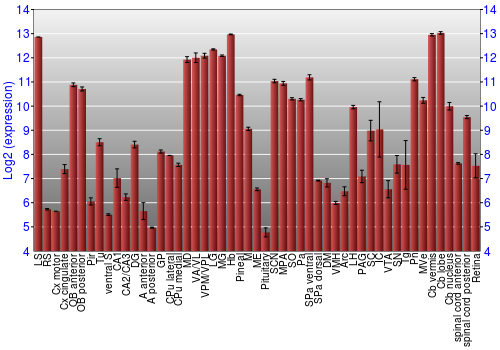
\includegraphics{exprgraph.png}
  \caption{exprgraph}
\end{figure}

\begin{figure}
  \centering
  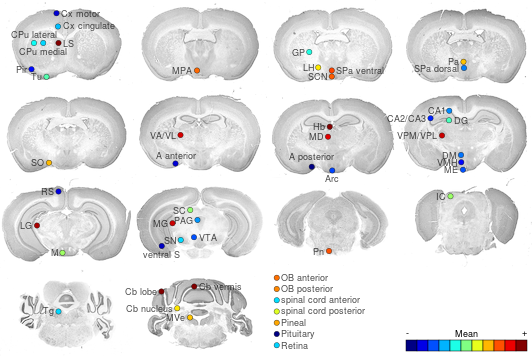
\includegraphics{exprmap.png}
  \caption{exprmap}
\end{figure}

\subsection{Keyword search}
The function \Rfunction{getBrainStars} provides keyword search in BrainStars. This function retrives a gene list or count of genes.
\begin{Schunk}
\begin{Sinput}
> recep.rjson <- getBrainStars("receptor/10,5")
> recep.count <- getBrainStars("receptor/count")
\end{Sinput}
\end{Schunk}
The useful ready-to-made functions were provided to extract "gene names", "gene symbols" and "probeset ids" from \Rpackage{RJSON} character object.
\begin{Schunk}
\begin{Sinput}
> recep.gns <- geneNames(recep.rjson)
> recep.gss <- geneSymbols(recep.rjson)
> recep.ids <- probeSetIDs(recep.rjson)
\end{Sinput}
\end{Schunk}
See detail about query format in next section.

\subsection{Getting a list of genes}
BrainStars has results of some higher-order biological anlaysis. You can retrive these information in following functions.

\subsubsection{Markers}
Marker genes were ones whose levels in a specific CNS region are higher (or lower) than in others.
\begin{Schunk}
\begin{Sinput}
> mk.genes.count <- getBrainStarsMarker("high/LS/count")
\end{Sinput}
\end{Schunk}
\subsubsection{Multistate and onestate genes}
Multi-state genes are ones with multi-modal expression patterns (i.e. expression of discretized states) or multi-modal patterns. For each probeset, CNS regions were grouped into the several "states" according to their expression values with variational Bayesian inference to fit to a gaussian mixture model. Multi-state genes, which have two or more states, were shown in the list. one-state genes, which have only one state, were not shown.
\begin{Schunk}
\begin{Sinput}
> ms.genes.list <- getBrainStarsMultistate("low/SCN/all")
\end{Sinput}
\end{Schunk}

One-state genes are expressed unimodally across the CNS regions, and approximately followed a log-normal distribution. Some one-state genes exhibited stable expression patterns, characterized by the log-normal distribution with a small variance, whereas others had more variable expression and showed the log-normal with a larger variance.
\begin{Schunk}
\begin{Sinput}
> os.genes.count <- getBrainStarsOnestate("count")
\end{Sinput}
\end{Schunk}

\subsubsection{Retrive a gene list by genes by gene family / categories}
The function provides lists of genes in gene families or in a gene categories. 
\begin{Schunk}
\begin{Sinput}
> gfc.genes1.count <- getBrainStarsGeneFamCat("tf//count")
> gfc.genes2.list <- getBrainStarsGeneFamCat("tf/terminal/all")
> gfc.genes3.count <- getBrainStarsGeneFamCat("tf/terminal/count")
\end{Sinput}
\end{Schunk}

\subsubsection{Inferred connections among CNS regions by neurotransmitter/neurohormone}
In the CNS, various neurohormones (NHs) and neurotransmitters (NTs) are secreted from neurons to convey information among distinct regions. The function get inferred interconnections among CNS regions by expression data (especially multi-state expression) for NH and NT (NH/NT) genes. To analyze the expression patterns of the NH/NT genes, a list that included the genes for the ligands themselves and those for enzymes that were rate-limiting in the biosynthesis of these ligands was first made. Here both of these categories were termed as "ligand" genes. the genes for NH/NT receptor proteins (i.e., "receptor" genes) were also included. Next, a list of connection among CNS regions that a state of a ligand gene of a NH/NT is "on" (or "up") in one region, and a state of a receptor gene of the NH/NT is "on" (or "up") in the other region was made.
\begin{Schunk}
\begin{Sinput}
> os.genes <- getBrainStarsNtNh("high/SCN/ME/all")
\end{Sinput}
\end{Schunk}

\section{BrainStars Web API} 
The BrainStars database has a REST-like Web API interface for accessing from your Web applications. This document shows how to access the database via our Web API. We have the following Web APIs:

\begin{itemize}
  \item Search API
  \item List API
  \item Probe set API
\end{itemize}

You can get contents in HTML, JSON, YAML, and so on. (See below)

\subsection{Search API}
Search API is for keyword search and is based on Tokyo Manifesto and TogoWS REST interface. URL for retrieving a list of hit entries:

\begin{verbatim}
http://brainstars.org/search/(query+string)[/(offset),(limit)]
\end{verbatim}

If the result has at least one hit entries, a list of entry IDs is returned in text/plain format (each line corresponds to each hit entry). If not, 404 Not found error code is returned. The output format can be changed to JSON, and so on (see below). "offset,limit" can be used to retrieve a part of hit entries. If "offset,limit" is not given, all hits are returned.

URL for retrieving the count of hit entries:
\begin{verbatim}
http://brainstars.org/search/(query+string)/count
\end{verbatim}

The count of hit entries is returned in text/plain format.

\subsubsection{Samples}
\begin{verbatim}
http://brainstars.org/search/receptor
http://brainstars.org/search/receptor/1,5
http://brainstars.org/search/receptor/count
\end{verbatim}

\subsection{List API}
List API is for retrieving a list of entries, such as genes in a specific gene category.

\begin{verbatim}
http://brainstars.org/(type)[/(category)[/(subcategory)[/...]]]/(offset),(limit)
http://brainstars.org/(type)[/(category)[/(subcategory)[/...]]]/all 
http://brainstars.org/(type)[/(category)[/(subcategory)[/...]]]/count
\end{verbatim}

You can specify "type" in the following list:
\begin{itemize}
  \item "marker": marker gene candidates
  \item "multistate": multi-state genes
  \item "onestate": one-state genes
  \item "ntnh": inferred connections among CNS regions by neurotransmitter/neurohormone
  \item "genefamily": gene family / categories
\end{itemize}

\subsubsection{Marker gene candidates (marker)}
List of entries and Count of entries: 
\begin{verbatim}
http://brainstars.org/marker/{high,low}/(region)/(offset),(limit) 
http://brainstars.org/marker/{high,low}/(region)/count 
\end{verbatim}

\begin{description}
  \item{\{high,low\}}
    \begin{itemize}
      \item "high": highly expressed regions
      \item "low": low expressed regions
    \end{itemize}        
  \item (region): CNS region
\end{description}    

\subsubsection{Multi-state genes (multistate)}
List of entries and Count of entries: 
\begin{verbatim}
http://brainstars.org/multistate/{high,up,low,down}/(region)/(offset),(limit) 
http://brainstars.org/multistate/{high,up,low,down}/(region)/count 
\end{verbatim}

\begin{description}
  \item{\{high,up,low,down\}}
    \begin{itemize}
      \item "high": high state regions
      \item "up": up state regions
      \item "low": low state regions
      \item "down": down state regions
    \end{itemize}
  \item{(region)} CNS region
\end{description}    

\subsubsection{One-state genes (onestate)}
List of entries and Count of entries: 
\begin{verbatim}
http://brainstars.org/onestate/(offset),(limit) 
http://brainstars.org/onestate/count
\end{verbatim}

\subsubsection{Inferred connections among CNS regions by neurotransmitter/neurohormone (ntnh)}
List of entries and Count of entries: 
\begin{verbatim}
http://brainstars.org/ntnh/{high,low}/(ligand-region)/(receptor-region)/(offset),(limit) 
http://brainstars.org/ntnh/{high,low}/(ligand-region)/(receptor-region)/count 
\end{verbatim}

\begin{description}
  \item{\{high,low\}}
    \begin{itemize}
      \item "high": high state regions
      \item "up": up state regions
    \end{itemize}        
  \item{(ligand-region)} Ligand CNS region
  \item{(receptor-region)} Receptor CNS region.
\end{description}

\subsubsection{Gene family / categories (genefamily)}
List of entries and Count of entries: 
\begin{verbatim}
http://brainstars.org/genefamily/(category)/(keyword)/(offset),(limit) 
http://brainstars.org/genefamily/(category)/(keyword)/count 
\end{verbatim}

\begin{description}
  \item{(category)} gene family / category name
    \begin{itemize}
      \item "tf": transcription factors
      \item "transmem": transmembrane genes
      \item "channel": channel genes
      \item "gpcr": GPCR genes
      \item "adhesion": cell adhesion genes
      \item "excellmat": extracellular matrix genes
      \item "structural": structural protein genes
      \item "neurogenesis": neurogenesis related genes
      \item "hox": homeobox genes
      \item "nucrcpt": nuclear receptor genes
      \item "ntnh": neurotransmitter/neurohormone genes
      \item "axon": axon guidance genes
      \item "fox": forkhead genes
  \end{itemize}
  \item{(keyword)} keyword. If no keyword search required, make this omited or blank  
\end{description}    

\subsubsection{Samples}
\begin{verbatim}
http://brainstars.org/marker/low/SCN/all
http://brainstars.org/multistate/up/SCN/20,10
http://brainstars.org/onestate/count
http://brainstars.org/ntnh/high/SCN/ME/all
http://brainstars.org/genefamily/tf//1,20
http://brainstars.org/genefamily/tf//count
http://brainstars.org/genefamily/tf/terminal/all
http://brainstars.org/genefamily/tf/terminal/count
\end{verbatim}

\subsection{Entry API}
Entry API is for obtaining information (annotation, expressions, links) about each entry
\begin{verbatim}
http://brainstars.org/probeset/(id)
\end{verbatim}

\subsubsection{Samples}
\begin{verbatim}
http://brainstars.org/probeset/1450371_at
http://brainstars.org/probeset/1450371_at?content-type=application/json
\end{verbatim}

\subsection{Content type}
How to designate a content type

You can get information in another format rather than default format (default: text/plain in search/list API; text/html in entry API).

Using a "content-type" parameter in the query string of the URI. 
\begin{verbatim}
http://brainstars.org/marker/high/LS?content-type=application/json
\end{verbatim}

Using an "Accept" header of your HTTP request. 
\begin{verbatim}
$ curl -H "Accept: application/json" http://brainstars.org/marker/high/LS 
$ wget --header "Accept: application/json" http://brainstars.org/marker/high/LS
\end{verbatim}

Supported content type:
\begin{itemize}
  \item JSON (text/x-json or application/json)
  \item YAML (text/yaml, text/x-yaml, or application/x-yaml)
  \item Perl Data::Dumper (text/x-data-dumper)
  \item Perl Data::Denter (text/x-data-denter)
  \item Perl Data::Taxi (text/x-data-taxi)
  \item Perl Storable (application/x-storable)
  \item Perl FreezeThaw (application/x-freezethaw)
  \item PHP Serialization (text/x-php-serialization)
\end{itemize}

\section{Conclusion}
The \Rpackage{BrainStars} package provides way to retrive gene expression, 
annotation and result of higher-order biological data analysis in R from 
BrainStars database. To perform many useful functions of Bioconductor, 
\Rpackage{BrainStars} package is adopted Bioconductor data structure, 
such a \Rclass{ExpressionSet}. These package will hopefully access BrainStars 
data more fully to the neuroscience community.
\end{document}
